\section{Properties of Wigner distributions}
\label{app:wigner}

Here we present important properties of the Wigner distribution that are used throughout the paper.

\begin{proposition}\label{thm:wstate}
  The Wigner distribution of a state $\rho \in \cal{B}(\cal{H}_d)$ is
  \begin{enumerate}
    \item[(i)]\label{en:w1} Real valued: $\W{\rho} \in \mathbb{R}^{d^2}$;
    \item[(ii)]\label{en:w2} Normalised: $\sum_{\bmz \in \cal{P}_d} \W[\bmz]{\rho}=1$;
    \item[(iii)]\label{en:w3} Bounded: $\abs{\W[\bmx]{\rho}} \leq \frac{1}{d}$.
    \item[(iv)]\label{en:w4} Additive under mixing: \vspace{2pt}\\
    $\W[\bmx]{\sum_i p_i \rho_i} = \sum\limits_i p_i \W[\bmx]{\rho_i}$;
    \item[(v)]\label{en:w5} Multiplicative under tensor products: \vspace{2pt}\\
    $\W[\bmx_A \oplus \bmx_B]{\rho_A \otimes \rho_B} = \W[\bmx_A]{\rho_A}\W[\bmx_B]{\rho_B}$.
	\end{enumerate}
\end{proposition}
Not all distributions satisfying these properties correspond to positive semi-definite states.
\begin{proof}
	\nick{Proof?}
\end{proof}

\begin{proposition}
    \label{thm:wchannel}
    The Wigner distribution of a $\cptp$ operation $\E: \cal{B}(\cal{H}_{d_A}) \mapsto \cal{B}(\cal{H}_{d_B})$ is
    \begin{enumerate}
        \item\label{en:wo1} Real-valued: $\W{\E} \in \mathbb{R}^{d^2} \times \mathbb{R}^{d^2}$;
        \item\label{en:wo2} Normalised: $\sum_{\bmz \in \cal{P}_{d_B}} \W[\bmz|\bmx]{\E} = 1$ \\ 
        for any $\bmx \in \cal{P}_{d_A}$;
        \item\label{en:wo3} Bounded: $\abs{\W[\bmy|\bmx]{\E}} \leq \frac{d_A}{d_B}$;
	    \item\label{en:wo4} Transitive: $\W[\bmy]{\E(\rho)} = \sum_{\bmz \in \cal{P}_{d_A}} \W[\bmy|\bmz]{\E} \W[\bmz]{\rho}$ for any $\bmy \in \cal{P}_{d_B}$.
    \end{enumerate}
\end{proposition}
If $d_A = d_B$, and in particular if operation $\E$ maps a Hilbert space onto itself, then the stochasticity condition $\abs{\W[\bmy|\bmx]{\E}} \leq 1$ is satisfied.
\begin{proof}
	\nick{Proof?}
\end{proof}
A $(d \times d)$ matrix $S$ is in $\stoch$, if
\begin{enumerate}
    \item $S_{ij} \geq 0$ for all $i, j \in \mathbb{Z}_d$;
    \item $\sum\limits_{j=1}^n S_{ij} = 1$ for all $i \in \mathbb{Z}_d$;
    \item $S\bmd = \bmd$.
\end{enumerate}

%%%%%%%%%%%%%%%%%%%%%%%%%%%%%%%%%%%%%%%%

\section{Properties of majorization}
\label{app:major}

\subsection{Simple--majorization equivalence conditions}

In the unital fragment, namely the limit of infinite temperature, $\beta = 0$, the free state is the maximally mixed state $\frac{1}{d}\id$ with uniform Wigner distribution $\frac{1}{d}\bm{1}  = (\frac{1}{d},\dots,\frac{1}{d})$.
This fragment is governed by simple majorization and we first prove strong equivalences for this type of majorization.
\begin{theorem}\label{thm:major}
Given $\bmx, \bmy \in \mathbb{R}^n$ the following statements are equivalent:
 \begin{enumerate}
	\item\label{en:m1} $\bmx \prec \bmy$;
	\item\label{en:m2} $\bmx = B \bmy$ for bistochastic $B$;
	\item\label{en:m3} $\sum\limits_{i=1}^n \abs{x_i - t} \leq \sum\limits_{i=1}^n \abs{y_i - t}$ for all $t \in \mathbb{R}$;
	\item\label{en:m4} $\sum\limits_{i=1}^n (x_i - t)^+ \leq \sum\limits_{i=1}^n (y_i - t)^+$ for all $t \in \mathbb{R}$ and $\sum\limits_{i=1}^n x_i = \sum\limits_{i=1}^n y_i$, where $(x)^+ = \max{\{x, 0\}}$;
	\item\label{en:m5} $L_{\bmx}(k) \leq L_{\bmy}(k)$ for $k=1,\dots,n-1$	and $L_{\bmx}(n) = L_{\bmy}(n)$.
 \end{enumerate}
\end{theorem}
\begin{proof}
	\nick{Proof?}
\end{proof}

\subsection{Embedding map}

Any $\bmd$-majorization problem can be rephrased as a simple majorization problem in a higher dimensional space via the embedding map.
\begin{definition}
  The embedding map $\Gamma_{\bmd}:\mathbb{R}^n \mapsto \mathbb{R}^D, D = \sum\limits_{i=1}^n d_i$ is the function
  \begin{equation}
    \Gamma_{\bmd}(\bmw) = \bigoplus_{i=1}^n w_i\  \frac{1}{d_i}\bm{1},
  \end{equation}
where $\bm{1}/d_i$ is the $d_i$-dimensional uniform distribution.
The left inverse $\Gamma_{\bmd}^{-1}: \mathbb{R}^D \mapsto \mathbb{R}^n$ is defined to sum up the elements in each block of $\Gamma_{\bmd}(\bmw)$, so that
  \begin{equation}
     \Gamma_{\bmd}^{-1}(\oplus_{i=1}^n w_i \bm{1}/d_i) = \bmw.
  \end{equation}
  This is not a right inverse, because $\Gamma_{\bmd}$ is not surjective.
\end{definition}
The direct sum simply amounts to listing the uniform distributions one after the other.
The embedding map maps the Gibbs distribution to the uniform distribution, $\Gamma_{\bmd}(\bmd) = \bm{1}/D$.
Then, a non-increasing ordering $\Gamma_{\bmd}(\bmz)^\downarrow$ in the new space, corresponds to the so-called ``$\beta$-ordering'' of the original vector denoted by the permutation $\pi$ in~\cref{def:lc}, mapping $(w_i/d_i) \mapsto (w_i/d_i)^\downarrow$ for all $i=1,\dots,n$.

\subsection{\textit{d}-majorization equivalence conditions}

\begin{theorem}
Given $\bmx, \bmy, \bmd \in \mathbb{R}^n$, such that the components of $\bmd$ are positive, the following statements are equivalent:
  \begin{enumerate}
    \item $\bmx \prec_{\bmd} \bmy$;
    \item $\Gamma_{\bmd}({\bmx}) \prec \Gamma_{\bmd}({\bmy})$;
    \item\label{en:tm3} $\sum\limits_{i=1}^n \abs{x_i - t d_i} \leq \sum\limits_{i=1}^n \abs{y_i - t d_i}$ for all $t \in \mathbb{R}$;
    \item $\sum\limits_{i=1}^n (x_i - t d_i)^+ \leq \sum\limits_{i=1}^n (y_i - t d_i)^+$ for all $t \in \mathbb{R}$ and $\sum\limits_{i=1}^n x_i = \sum\limits_{i=1}^n y_i$;
    \item $L_{\bmx|\bmd}(k) \leq L_{\bmy|\bmd}(k)$ for $k=1,\dots,n-1$	and $L_{\bmx|\bmd}(n) = L_{\bmy|\bmd}(n)$.
  \end{enumerate}
\end{theorem}
\begin{proof}
  \nick{Proof?}
\end{proof}
\iffalse
    \begin{enumerate}
        \item[1$\leftrightarrow2$]
        Suppose now there exists a stochastic $S$ such that $\bmx = S\bmy$ with $\bmd = S\bmd$ and let $B = \Gamma_{\bmd} \circ S \circ \Gamma_{\bmd}^{-1}$.
        $B$ is a $D$-dimensional bistochastic matrix, since composition of stochastic matrices is stochastic and $(\Gamma_{\bmd} \circ S \circ \Gamma_{\bmd}^{-1}) (\frac{1}{D}\bm{1}) = (\Gamma_{\bmd} \circ S) (\bm{d}) = \Gamma_{\bmd}(\bm{d}) = \frac{1}{D}\bm{1}$. Then, $B$ maps $\Gamma_{\bmd}({\bmy})$ to $\Gamma_{\bmd}({\bmx})$.
        Conversely, given $B$, let $S = \Gamma_{\bmd}^{-1} \circ B \circ \Gamma_{\bmd}$.
        Similarly, $S$ is the stochastic matrix that preserves $\bmd$ and maps $\bmy$ to $\bmx$.
        \item[$2\leftrightarrow3$]\hspace{-5pt}, $2\leftrightarrow4$, $2\leftrightarrow5$ These three statement are equivalent to \nick{blah} respectively for the embedded vectors $\Gamma_{\bmd}({\bmx}), \Gamma_{\bmd}({\bmy})$.
        This is clear by rewriting
        \begin{align}
            \sum\limits_{i=1}^n \abs{x_i - t d_i} &= \sum\limits_{i=1}^n d_i \abs{\frac{x_i}{d_i} - t} = \sum\limits_{i=1}^D \abs{\Gamma_{\bmd}(\bmx)_i - t}, \\
            \sum\limits_{i=1}^n (x_i - t d_i)^+ &= \sum\limits_{i=1}^D (\Gamma_{\bmd}(\bmx)_i - t)^+, \\
            L_{\bmx|\bmd}(k) &= L_{\Gamma_{\bmd}(\bmx)}(k'), \\
            \text{with}\ k&=1,\dots,n\ \text{and}\ k'=1,\dots,D \nonumber
        \end{align} 
        and similarly for the right hand side.
    \end{enumerate}
\fi

%%%%%%%%%%%%%%%%%%%%%%%%%%%%%%%%%%%%%%%%

\section{Technical properties of $\sigma$--fragments}
\label{app:frag}

\nick{this section hasn't been refereced in various parts of the main text}

\begin{theorem}\label{thm:frag_app}
    Let $\R_\sigma = (\O_\sigma, \F_\sigma)$ be a $\sigma$--fragment of magic theory $\R = (\O, \F)$. 
    The following statements hold:
    \begin{enumerate}
        \item No $\sigma$--fragment is empty.
        \item If a free operation leaves two states invariant, then it also leaves their mixtures invariant, 
        \begin{equation*}
            \O_{\sigma} \cap \O_{\sigma'} \subseteq \O_{p\sigma + (1-p)\sigma'}\ \text{for all}\ p \in [0,1].
        \end{equation*}
        \item Let $\E$ be a $\cptp$ operation with Wigner distribution $\W{\E}$.
        For $\R = \Rmax$, $\E \in \O_\sigma$ iff $\W{\E} \in \stochw$. \nick{I don't like this one}
    \end{enumerate}
\end{theorem}
\begin{proof}$ $\\

    \begin{enumerate}
    \item The identity channel $1_{\rm{C}}: \D \mapsto \D$ belongs to every $\sigma$--fragment, as $1_{\rm{C}} \in \O$ and $1_{\rm{C}}\sigma = \sigma$ for all $\sigma \in \F$.
    
    \item Let $\E \in \O_{\sigma} \cap \O_{\sigma'}$.
    Then $\E \in \cptp$ and corresponds to stochastic Wigner distribution $\W{\E}$ such that $\W{\E} \W{\sigma} = \W{\sigma}$ and $\W{\E} \W{\sigma'} = \W{\sigma'}$.
    Then, $\W{\E} \W{p\sigma + (1-p)\sigma'} = \W{p\sigma + (1-p)\sigma'}$ for any $p \in [0,1]$ due to the additive property~\ref{en:w4} of the Wigner distribution, implying that state $p\sigma + (1-p)\sigma'$ is also left invariant by $\E$.
    
    \item Let $\O_\sigma' \coloneqq \{ \E \in \cptp: \W{\E} \in \stochw \}$ be the described set of operations.
    
    Suppose $\E$ is in $\O_\sigma$, then $\E \in \cptp$ and $\W{\E} \in \stochw$ due to property~\ref{en:wo4} of~\cref{thm:wchannel}, hence $\O_\sigma \subseteq \O_\sigma'$.
    
    Conversely, suppose $\E \in \cptp$ with $\W{\E} \in \stochw$. 
    Then, $\W[\bmy|\bmx]{\E} \geq 0$ for all $\bmx, \bmy$, hence $\E \in \O$.
    Furthermore, $\W{\E} \W{\sigma} = \W{\sigma}$ implies $\E(\sigma) = \sigma$ using~\cref{eq:woperation} defined for any $\cptp$ operation $\E$.
    Hence, $\O_\sigma' \subseteq \O_\sigma$.
    \end{enumerate}
\end{proof}

Any free state $\sigma \in \F$ corresponds to a $d^2$-dimensional probability distribution $\W{\sigma}$ and any free operation $\E \in \O$ corresponds to a $d^2 \times d^2$ stochastic matrix (or conditional probability distribution) $\W{\E}$.
Note that these mappings are one-to-one due to the orthogonality of the phase-point operators as an operator basis.

Note further that free states $\F$ are mapped onto a \emph{strict subset} of the set of probability distributions.
As a counterexample, the sharp $d^2$-dimensional probability distribution $(1, 0, \dots, 0)$ does not correspond to any qudit Wigner distribution because of the boundedness condition in~\cref{thm:wstate}.

Similarly, not all stochastic matrices correspond to completely positive operations.
As an example, consider the permutation matrix
\begin{equation}
    \Pi_X = \begin{psmallmatrix}
        0 & 1 & 0 & 0 & 0 \\
        0 & 0 & 0 & 0 & 1 \\
        0 & 0 & 0 & 1 & 0 \\
        1 & 0 & 0 & 0 & 0 \\
        0 & 0 & 1 & 0 & 0
    \end{psmallmatrix} \otimes \begin{psmallmatrix}
        0 & 0 & 1 & 0 & 0 \\
        0 & 0 & 0 & 0 & 1 \\
        0 & 0 & 0 & 1 & 0 \\
        1 & 0 & 0 & 0 & 0 \\
        0 & 1 & 0 & 0 & 0    
    \end{psmallmatrix} \in {\rm{S}}_5({\W{\frac{1}{5}\id}}).
\end{equation}
It preserves the uniform distribution $\W{\frac{1}{5}\id}$, but it does not correspond to any positive (hence quantum) operation.

%%%%%%%%%%%%%%%%%%%%%%%%%%%%%%%%%%%%%%%%

\section{Properties of Lorenz curves}
\label{app:lc_properties}

\nick{Prove statements underneath~\cref{def:lc}?}

\subsection{Basic properties}

Furthermore, single-copy Lorenz curves are simply additive in noise, 
\begin{equation}
	\lc{(1-\epsilon)\rho + \epsilon\sigma}{\sigma} = (1-\epsilon)\lc{\rho}{\sigma} + \epsilon\lc{\sigma}{\sigma},
\end{equation}
for any $\sigma, \rho$.
This is not true for higher number of copies.

\subsection{$\sigma$--fragment continuity}

\begin{proposition}\label{thm:lccont}
	The Lorenz curve $\lc{\rho}{\sigma}(x)$ of a state $\rho$ with respect to state $\sigma$ is uniformly continuous in $\sigma$.
\end{proposition}
\begin{proof}
	\nick{Idea:} If $\sigma$ and $\sigma'$ are $\delta$-close with respect to a state norm, then the curves $\lc{\rho}{\sigma}(x)$ and $\lc{\rho}{\sigma'}(x)$ are $\epsilon$-close at all $x \in [0,1]$.
\end{proof}

\subsection{Area monotone}\label{app:areamono}

\nick{I don't believe in the area monotone - should we keep?}

\begin{figure}[h]%
    \centering
    \subfigure[][]{%
    \label{fig:test1}%
    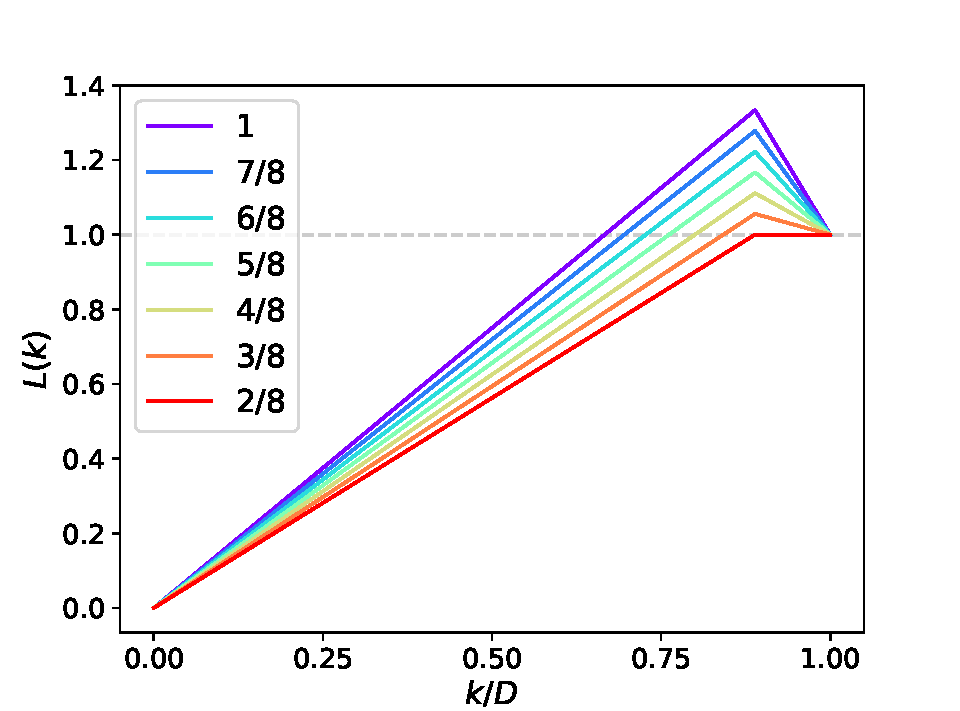
\includegraphics[height=3cm]{figs/negmasking_rho_strange_lc.pdf}
    %\caption{Maximally mixed state $\frac{1}{3}\id$}%
    }\hspace{8pt}%
    \subfigure[][]{%
    \label{fig:test2}%
    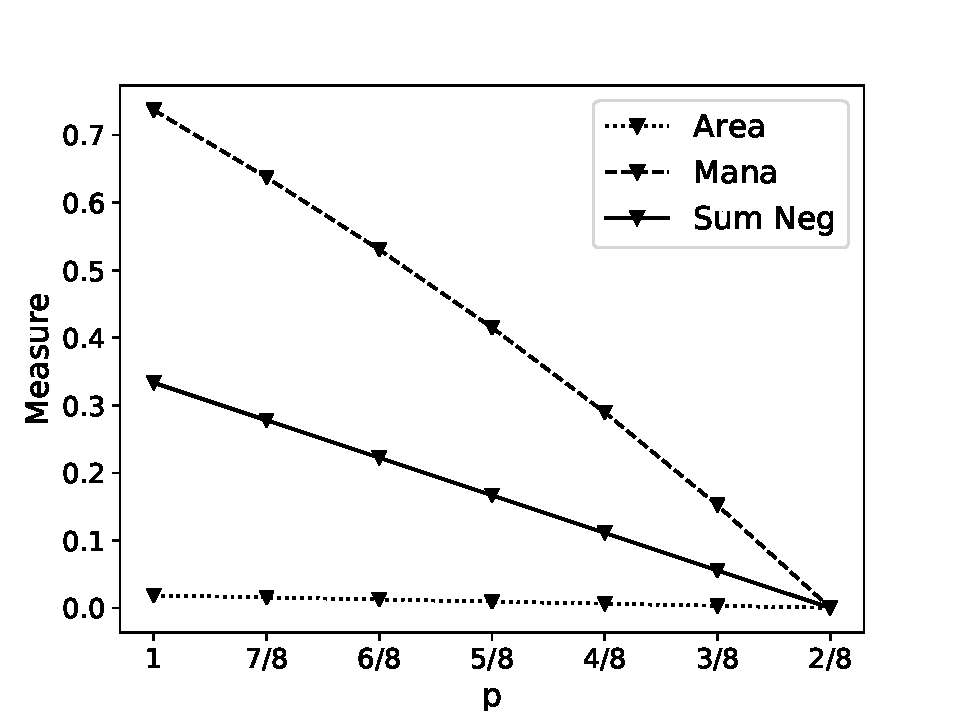
\includegraphics[height=3cm]{figs/negmasking_rho_strange_meas.pdf}
    %\caption{Zero state $\ketbra{0}{0}$}%
    }
    \caption{\subref{fig:test1} Lorenz curve of $p\ketbra{\rm{S}} + (1-p) \frac{1}{d}\id$ for $p$ given in the legend.\subref{fig:test2} Different measures for the states on the left. \\
    \nick{can replace~\cref{fig:lctoy} with a more informative version of this figure}
    }%
    \label{fig:test}
\end{figure}

Let $L_{>1}$ be the set of points on the Lorenz curve $\lc{\rho}{\sigma}(k)$ that lie above $1$ of state $\rho$ in the $\sigma$--fragment. 
If $\rho$ is a free state, $L_{>1}$ is empty and $\A_\sigma(\rho) = 0$. 
Otherwise, $\A_\sigma(\rho) > 0$ and it can be calculated exactly using the trapezium rule or the shoelace formula. 
Let $k$ be the index of the first point $\left(x_k, \lc{\rho}{\sigma}(k)\right)$ lying above $1$. 
Then $L_\rho(k)$ crosses $1$ at
\begin{equation}
	x_{\rm{int}} = x_k - \frac{x_k - x_{k-1}}{\lc{\rho}{\sigma}(k) - \lc{\rho}{\sigma}(k-1)}\lc{\rho}{\sigma}(k),\vspace{10pt}
\end{equation}
as well as at $\left(x_d, \lc{\rho}{\sigma}(d)\right) = (1,1)$

Now we can define
\begin{equation}
L_{>1}^+ = \{ (x_i, y_i) \}_{0 \leq i \leq n}
\end{equation}
such that it contains the initial point of intersection $(x_0, y_0) \equiv (x_{n+1}, y_{n+1}) \coloneqq (x_{\rm{int}}, 1)$, all points $(x_i, y_i)$, labelled by $i=1,\dots,n-1$ that lie above $y=1$ contained in $L_{>1}$ and finally the second point of intersection $(x_n, y_n) = (1,1)$.
Then, 
\begin{equation}
	\A_\sigma(\rho) = \frac{1}{2} \sum\limits_{i=0}^n (x_{i+1} y_i - x_i y_{i+1}).
\end{equation}

\subsection{Lorenz curve independent constraints}\label{app:lc_constraints}

\begin{theorem}\label{thm:elbows}
	Let $\rho, \tau$ be two quantum states with Lorenz curves $\lc{\rho}{\sigma}(x), \lc{\tau}{\sigma}(x)$ in the $\sigma$--fragment.
	
	Let $t$ be the number of elbows of $\lc{\tau}{\sigma}(x)$ at locations $x_1, \dots, x_t$.
	
	Then, $\lc{\rho}{\sigma}(x) \geq \lc{\tau}{\sigma}(x)$ for all $x \in [0,1]$ iff $\lc{\rho}{\sigma}(x_{i}) \geq \lc{\tau}{\sigma}(x_{i})$ for all $i =1,\dots,t$.
\end{theorem}
\begin{proof}	
	$\lc{\rho}{\sigma}(x) \geq \lc{\tau}{\sigma}(x)$ for all $x \in [0,1]$ trivially implies $\lc{\rho}{\sigma}(x_{i}) \geq \lc{\tau}{\sigma}(x_{i})$ for all $i = 1,\dots,n'$.
	
	Conversely, assume that $\lc{\rho}{\sigma}(x_{i}) \geq \lc{\tau}{\sigma}(x_{i})$ for all $i = 1,\dots,r$.
	First, let $x_0 = 0$ and $x_{n'+1} = 1$, so that $\lc{\rho}{\sigma}(x_0) = \lc{\tau}{\sigma}(x_0) = 0$ and $\lc{\rho}{\sigma}(x_{n'+1}) = \lc{\tau}{\sigma}(x_{n'+1}) = 1$.
	Hence, we can extend the set of elbows $E$ to $E' = E \cup \{x_0, x_{n'+1}\}$.
	
	Pick two consecutive locations $x_{i}, x_{i+1}$ in $E'$ and consider the line segment $\ell_\tau(x)$ connecting points $(x_{i}, \lc{\tau}{\sigma}(x_{i}))$ and $(x_{i+1}, \lc{\tau}{\sigma}(x_{i+1}))$ as well as the line segment $\ell_\rho(x)$ connecting points $(x_{i}, \lc{\rho}{\sigma}(x_{i}))$ and $(x_{i+1}, \lc{\rho}{\sigma}(x_{i+1}))$.
	This is illustrated in~\cref{fig:elbows_proof}.
\begin{figure}[h]
    \centering
    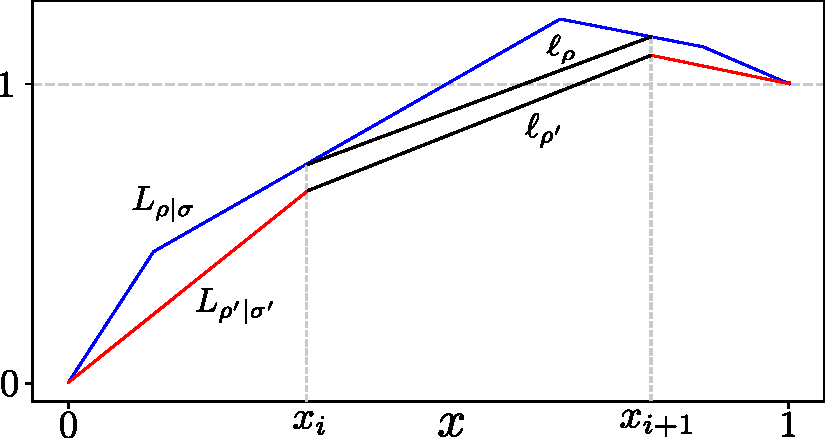
\includegraphics[scale=0.6]{figs/elbows_proof.pdf}
    \caption{\textbf{Illustration of~\cref{thm:elbows}}.
    }
    \label{fig:elbows_proof}
\end{figure}

	Due to concavity of $\lc{\rho}{\sigma}$, it is clear that for all $x \in [x_{i}, x_{i+1}]$, we have $\lc{\rho}{\sigma}(x) \geq \ell_\rho(x) \geq \ell_\tau(x) = \lc{\tau}{\sigma}(x)$.
	This argument can be made in all intervals $[x_{i}, x_{i+1}]$ with $i=0,\dots,n'$, so the proof is complete.
\end{proof}
This theorem is of practical importance in calculating the necessary distillation constraints derived via majorization.

\nick{In particular}, it can be used in the discussion of standard Lorenz curves to set the necessary constraints,
\begin{align}
L\left(x_{I'(0, m'_{0}, 9^{n-n'})}\right) &\geq L\left(x_{I'(0, m'_{0}, 9^{n-n'})}\right), \nonumber\\
L\left(x_{I'(1, m'_{1}, 9^{n-n'})}\right) &\geq L\left(x_{I'(1, m'_{1}, 9^{n-n'})}\right), \nonumber\\
&\vdotswithin{=} \nonumber\\
L\left(x_{I'(n', m'_{r}, 9^{n-n'})}\right) &\geq L\left(x_{I'(n', m'_{n'}, 9^{n-n'})}\right), \nonumber
\end{align}
where $x_{I'(0, m'_{0}, 9^{n - n'})}, x_{I'(1, m'_{1}, 9^{n - n'})}, \dots, x_{I'(n', m'_{n'}, 9^{n - n'})} \in T$ are the locations of the elbows of $\lc{\rho_{\rm{S}}(\epsilon')^{\otimes n'}}{\frac{1}{d}\id}$ (excluding $0$ and $1$).

%%%%%%%%%%%%%%%%%%%%%%%%%%%%%%%%%%%%%%%%

\section{Technical derivation for Lorenz curves in unital fragment}
\label{app:lcsu_technical}

\subsection{Binomial distributions and error bounds}\label{app:phi}
Consider an experiment consisting of $n$ trials of throwing a $p$-coin, that is a coin with probability $p$ of landing on one side and $1-p$ of landing on the other.
This scenario describes the construction of an $n$-copy Strange state Wigner distribution from a single-copy as presented in~\cref{sec:lcsu}.
The experiment is described by binomial statistics and we write down the sum over an even number of successful trials $\Phi_+$ (over an odd number of successful trials $\Phi_-$),
\begin{align}	
	\Phi_+(af; nf, p) &\coloneqq \sum\limits_{\ell=0}^{af/2} \binom{nf}{2\ell} p^{2\ell} (1-p)^{nf-2\ell}, \nonumber\\ 
	&\text{for even integers } af\in[0,nf], \label{eq:fp_app} \\
	\Phi_-(af; nf, p) &\coloneqq \sum\limits_{\ell=1}^{(af-1)/2} \binom{nf}{2\ell+1} p^{2\ell+1} (1-p)^{nf-(2\ell+1)}, \nonumber\\ 
	&\text{for odd integers } af\in[0,nf]. \label{eq:fn_app}
\end{align}
Note that index $af$ only takes even (odd) values when labelling $\Phi_+$ ($\Phi_-$).
In~\cref{app:lcsu_coord_elb}, we will use $\Phi_+$ and $\Phi_-$ to express the elbow coordinates of standard Lorenz curves.

We define the classical entropy of a $p$-coin as well as the classical relative entropy between a $p$-coin and a $q$-coin,
\begin{align}
	S(p) &\coloneqq -p\log{p} -(1-p)\log{(1-p)}, \label{eq:ent}\\
	\ent{p}{q} &\coloneqq p \log{\frac{p}{q}} + (1-p) \log{\frac{1-p}{1-q}}. \label{eq:ent_rel}
\end{align}
They are symmetric in the sense that $S(p) = S(1-p)$ and $\ent{p}{q} = \ent{1-p}{1-q}$.

A useful result is the entropic bound on a combination~\cite{cit:ash}.
\begin{lemma}\label{lem:comb_bounds}
	For all $\ell\in [1,np-1]$,
	\begin{align}
		&\left[ 8\ell\left(1-\frac{\ell}{np}\right) \right]^{-\frac{1}{2}} 2^{n S\left(\frac{\ell}{np}\right)} \leq \binom{np}{\ell} \leq \\
		&\left[ 2\pi \ell\left(1-\frac{\ell}{np}\right) \right]^{-\frac{1}{2}} 2^{n S\left(\frac{\ell}{np}\right)}.
	\end{align}
\end{lemma}
\begin{proof}
	For $\ell = 1,2, np-1, np-2$ check by direct calculation.	
	For all other cases, use Stirling's approximation. 
	\nick{CITE}
\end{proof}
With the help of this lemma, we directly arrive at 
\begin{theorem}\label{thm:bounds_strict}
	Given fixed $n>0$ and $p$, $\Phi_+, \Phi_-$ satisfy the following bounds:
	\begin{align*}
		\begin{split}
		&\text{1. } \Phi_+(a; n, p) \geq \sum\limits_{\ell=0}^{np/2}\left[ 16\ell\left(1-\frac{2\ell}{np}\right) \right]^{-\frac{1}{2}} 2^{-n\ent{\frac{2\ell}{nf}}{p}}, \\
		&\hspace{14pt} \text{for all even } a\in [2,np] \\
		&\text{2. } \Phi_+(a; n, p) \leq \sum\limits_{\ell=0}^{np/2}\left[ 4\pi\ell\left(1-\frac{2\ell}{nf}\right) \right]^{-\frac{1}{2}} 2^{-n\ent{\frac{2\ell}{np}}{p}}, \\
		&\hspace{14pt} \text{for all even } a\in [2,np] \\
		&\text{3. } \Phi_-(a; n, p) \geq \sum\limits_{\ell=1}^{(np-1)/2}\left[ 16(\ell+1)\left(1-\frac{2\ell+1}{np}\right) \right]^{-\frac{1}{2}} \times \\
		&\hspace{14pt} \times 2^{-n\ent{\frac{2\ell+1}{np}}{p}},\ \text{for all odd }a\in [1,np] \\
		&\text{4. } \Phi_-(a; n, p) \leq \sum\limits_{\ell=1}^{(np-1)/2}\left[ 4\pi(\ell+1)\left(1-\frac{2\ell+1}{nf}\right) \right]^{-\frac{1}{2}} \times \\
		&\hspace{14pt} \times 2^{-n\ent{\frac{2\ell+1}{np}}{p}},\ \text{for all odd } a\in [1,np]
		\end{split}
	\end{align*}
\end{theorem}
\begin{proof}
	All four statements follow from application of~\cref{lem:comb_bounds} on the combinatorial coefficient and the defintion of relative entropy given in~\cref{eq:ent_rel}
\end{proof}

\iffalse % LOOSE BOUNDS & PLOT - START
The experiment is described by binomial statistics and we define the left tail of the cumulative binomial distribution,
\begin{equation}\label{eq:phil}
	\Phi_\ell(m; n, p) \coloneqq \sum\limits_{j=0}^m \binom{n}{j} p^j (1-p)^{n-j},
\end{equation}
where $m\in [0,n]$. 

The symmetry between the left tail of a $p$-coin distribution and the right tail of a $(1-p)$-coin distribution dictates that
\begin{align}\label{eq:phi_reverse}
	\Phi_\ell(m; n, p) + \Phi_\ell(n-m-1; n, 1-p) &= 1,\ m\in [0,n-1],
\end{align}
Entropic bounds on $\Phi_\ell$~\cite{cit:ash}.
\begin{lemma}\label{lem:phil_bounds}
	Given fixed $n>0$ and $p$, $\Phi_\ell$ satisfies the following bounds:
	\begin{align*}
		\begin{split}
		&\text{1. } \Phi_\ell(m; n, p) \geq \left[ 8m\left(1-\frac{m}{n}\right) \right]^{-\frac{1}{2}} 2^{-n\ents},\ m\in [1,n-1] \\
		&\text{2. } \Phi_\ell(m; n, p) \leq 2^{-n\ents},\ m\in [0,np] \\
		&\text{3. } \Phi_\ell(m; n, p) \leq 1 - \left[ 8(m+1)\left(1-\frac{m+1}{n}\right) \right]^{-\frac{1}{2}} 2^{-n\ent{\frac{m+1}{n}}{p}}, \\
		&\hspace{14pt} m\in [0,n-2]
		\end{split}
		\\
		&\text{4. } \Phi_\ell(m; n, p) \geq 1 - 2^{-n\ent{\frac{m+1}{n}}{p}},\ m\in [np+1,n-2]
	\end{align*}
\end{lemma}
\begin{proof}
	\nick{cite proof}
\end{proof}
Loose bounds follow
\begin{lemma}\label{lem:bounds_loose}
	Given fixed $n>0$ and $p$, $\Phi$ satisfies the following bounds:
	\begin{align*}
		\begin{split}
		&\text{1. } \Phi_{\pm}(m; n, p) \geq \left[ 8m\left(1-\frac{m}{n}\right) \right]^{-\frac{1}{2}} 2^{-n\ents},\ m\in [1,n-1] \\
		&\text{2. } \Phi_{\pm}(m; n, p) \leq 2^{-n\ents},\ m\in [0,np] \\
		&\text{3. } \Phi_{\pm}(m; n, p) \leq 1 - \left[ 8(m+1)\left(1-\frac{m+1}{n}\right) \right]^{-\frac{1}{2}} 2^{-n\ent{\frac{m+1}{n}}{p}}, \\
		&\hspace{14pt} m\in [0,n-2]
		\end{split}
	\end{align*}
\end{lemma}
\begin{proof}
	\nick{paste proof}
\end{proof}

We can therefore use~\cref{lem:bounds_loose,lem:bounds_strict} to bound the standard Lorenz curves.
\begin{figure}[b]
    \centering
    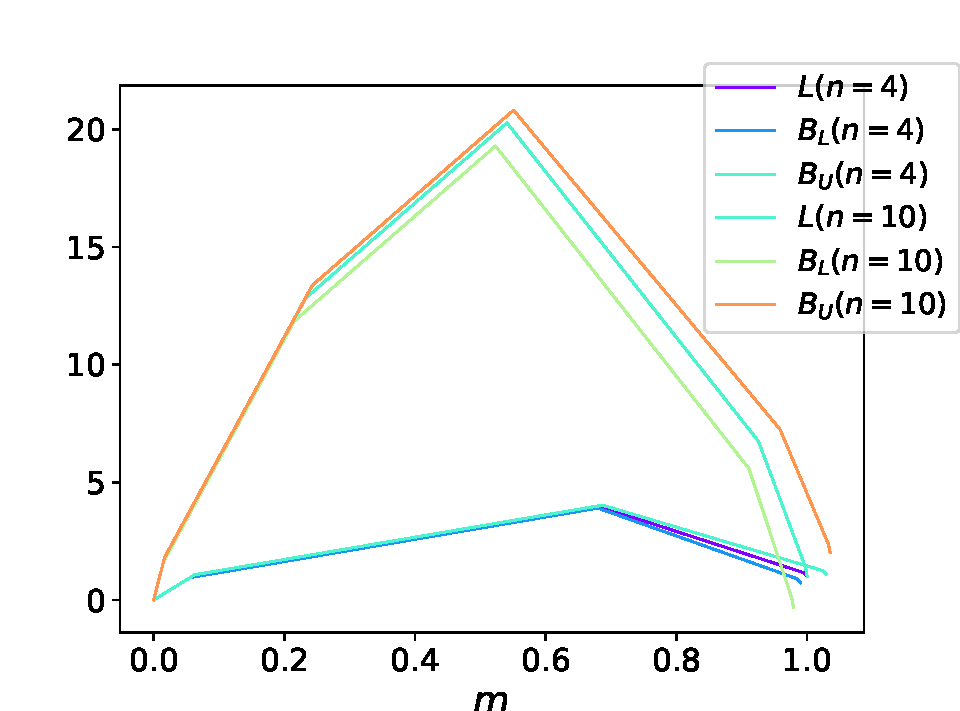
\includegraphics[scale=0.4]{figs/lc_bounds.pdf}
    \caption{\textbf{Lorenz curves and bounding curves.} 
    The figure explores the distillation process of a 10-copy $0.25$-noisy Strange state to a 4-copy $0.05$-noisy Strange state in the unital fragment.
    Clearly, by looking at the Lorenz curves, the distillation process is possible.
    However the bounding curves, derived in~\cref{lem:bounds_strict}, intersect at the end, suggesting that the process is not necessarily possible.
    }
    \label{fig:lc_bounds}
\end{figure}
\fi % LOOSE BOUNDS & PLOT - END

\subsection{Standard Lorenz curve elbow coordinates}\label{app:lcsu_coord_elb}
The Wigner distribution of the $n$-copy qutrit maximally mixed state $\left(\id/3\right)^{\otimes n}$ is the uniform distribution 
\begin{equation}\label{eq:wu}
	\W{\left(\id/3\right)^{\otimes n}} = \Bigg( \overbrace{\frac{1}{9^n}, \dots, \frac{1}{9^n}}^{9^n} \Bigg).
\end{equation}
The Wigner distribution of the 1-copy $\epsilon$-noisy Strange state $\rho_{\rm{S}}(\epsilon)$ in the unital fragment is a permutation of 
\begin{equation}\label{eq:wsu}
	\W{\rho_{\rm{S}}(\epsilon)} = \Bigg( \overbrace{\frac{1}{6} - \frac{1}{18}\epsilon, \dots, \frac{1}{6} - \frac{1}{18}\epsilon}^8, \overbrace{-\frac{1}{3} + \frac{4}{9}\epsilon}^1 \Bigg)
\end{equation}
The two distinct components are plotted~\cref{fig:noisys} as a function of noise. 
It is clear that in the unital fragment the Strange state contains Wigner negativities in the regime $0 \leq \epsilon \leq \tfrac{3}{4}$.
\begin{figure}[h]
    \centering
    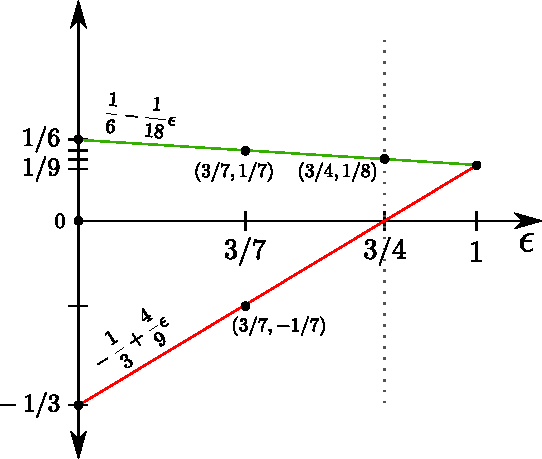
\includegraphics[scale=0.7]{figs/noisys.pdf}
    \caption{\textbf{Wigner components of the noisy Strange state.} 
    In the interval $0 \leq \epsilon < 3/7$, the negative component is larger than the positive components.
    At $\epsilon = 3/7$ the Wigner distribution is $(-\frac{1}{7},\frac{1}{7},\dots,\frac{1}{7})$.
    In the interval $3/7 < \epsilon < 3/4$, the positive components are larger than the negative component.
    In the interval $3/4 \leq \epsilon \leq 1$, there is no negativity.
    }
    \label{fig:noisys}
\end{figure}

The Wigner distribution of the $n$-copy $\epsilon$-noisy Strange state $\rho_{\rm{S}}(\epsilon)^{\otimes n}$ in the unital fragment is given by the convolution $\W{\rho_{\rm{S}}(\epsilon)^{\otimes n}} = \rm{W}_{\rho_{\rm{S}}(\epsilon)}^{\otimes n}$.
In general, $\rho_{\rm{S}}(\epsilon)^{\otimes n}$ contains $n + 1$ distinct components, labelled $0,\dots, n$.
We present the distinct Wigner components of $\rho_{\rm{S}}(\epsilon)^{\otimes n}$ along with their multiplicites in~\cref{tab:lcsu}.
Note that LHS (RHS) refers to elbow coordinates $i$ on the left of and including (right of) the maximum, precisely
\begin{align}
&\text{LHS: } 0 \leq i \leq \left\lfloor \frac{n}{2} \right\rfloor ; \\
&\text{RHS: } \left\lfloor \frac{n}{2} \right\rfloor +1 \leq i \leq n.
\end{align}
\begin{table}[h]
  \def\arraystretch{1.5}
  \centering
  \begin{tabular}{c|c|c|r|r}
    \multicolumn{3}{c|}{Case} & \multicolumn{1}{c}{$m_{i}(n, \epsilon)$} & \multicolumn{1}{|c}{$w_{i}(n, \epsilon)$} \\[0.5ex]\hline
    \multirow{4}{*}{\raisebox{-4ex}{\rotatebox[origin=c]{90}{$0\leq \epsilon < \frac{3}{7}$}}} & \hspace{0.8ex}\multirow{2}{*}{\raisebox{-1ex}{\rotatebox[origin=c]{90}{$n$ even}}}\hspace{0.8ex} & LHS & $8^{2i}\binom{n}{2i}$ & $\left( \frac{1}{6} - \frac{1}{18}\epsilon \right)^{2i}\left( -\frac{1}{3} + \frac{4}{9}\epsilon \right)^{n-2i}$ \\
    & & RHS & $8^{n-2i}\binom{n}{2i}$ & $\left( \frac{1}{6} - \frac{1}{18}\epsilon \right)^{n-2i}\left( -\frac{1}{3} + \frac{4}{9}\epsilon \right)^{2i}$ \\ \cline{2-5}
    & \multirow{2}{*}{\raisebox{-2ex}{\rotatebox[origin=c]{90}{$n$ odd}}} & LHS & $8^{2i+1}\binom{n}{2i+1}$ & $\left( \frac{1}{6} - \frac{1}{18}\epsilon \right)^{2i+1}\left( -\frac{1}{3} + \frac{4}{9}\epsilon \right)^{n-2i-1}$ \\
    & & RHS & $8^{n-2i-1}\binom{n}{2i+1}$ & $\left( \frac{1}{6} - \frac{1}{18}\epsilon \right)^{n-2i-1}\left( -\frac{1}{3} + \frac{4}{9}\epsilon \right)^{2i+1}$ \\ \hline
    \multirow{4}{*}{\raisebox{-4ex}{\rotatebox[origin=c]{90}{$\frac{3}{7}\leq \epsilon < \frac{3}{4}$}}} & \multirow{2}{*}{\raisebox{-1ex}{\rotatebox[origin=c]{90}{$n$ even}}} & LHS & $8^{n-2i}\binom{n}{2i}$ & $\left( \frac{1}{6} - \frac{1}{18}\epsilon \right)^{n-2i}\left( -\frac{1}{3} + \frac{4}{9}\epsilon \right)^{2i}$ \\
    & & RHS & $8^{2i}\binom{n}{2i}$ & $\left( \frac{1}{6} - \frac{1}{18}\epsilon \right)^{2i}\left( -\frac{1}{3} + \frac{4}{9}\epsilon \right)^{n-2i}$ \\ \cline{2-5}
    & \multirow{2}{*}{\raisebox{-2ex}{\rotatebox[origin=c]{90}{$n$ odd}}} & LHS & $8^{n-2i}\binom{n}{2i}$ & $\left( \frac{1}{6} - \frac{1}{18}\epsilon \right)^{n-2i}\left( -\frac{1}{3} + \frac{4}{9}\epsilon \right)^{2i}$ \\
    & & RHS & $8^{2i}\binom{n}{2i}$ & $\left( \frac{1}{6} - \frac{1}{18}\epsilon \right)^{2i}\left( -\frac{1}{3} + \frac{4}{9}\epsilon \right)^{n-2i}$ \\ \hline
  \end{tabular}
  \caption{Wigner components $w_{i}(n, \epsilon)$ of $\rho_{\rm{S}}(\epsilon)^{\otimes n}$ along with their multiplicities $m_{i}(n, \epsilon)$ in decreasing order in $i,\ 0 \leq i \leq n$.
  The order changes depending on the noise level $\epsilon$, the parity of the number of copies $n$ and the parity of the components (LHS vs RHS).
  Multiplication $2i$ is considered modulo $(n+1)$.}
  \label{tab:lcsu}
\end{table}

For example, the distribution of state $\rho_{\rm{S}}(0)^{\otimes 2}$ is
\begin{equation*}
	\begin{split}
	\rm{W}_{\rho_{\rm{S}}(0)^{\otimes 2}} = \Bigg( &\overbrace{\left( -\frac{1}{3} \right)^2}^1, \overbrace{\left( \frac{1}{6} \right)^2, \dots, \left( \frac{1}{6} \right)^2}^{64}, \\
	&\overbrace{ -\frac{1}{3} \cdot \frac{1}{6}, \dots, -\frac{1}{3} \cdot \frac{1}{6}}^{16} \Bigg)
	\end{split}
\end{equation*}

Every standard Lorenz curve contains $n$ elbows, labelled by 
\begin{equation*}
\{(x_{i}, L_{i})\}_{i=-1,0,\dots,n}\ ,
\end{equation*}
where the boundary points $(x_{-1}, L_{-1}) = (0,0)$ and $(x_{n}, L_{n}) = (1,1)$ are also included.
The maximum is the $(\lfloor n/2 \rfloor)$-th elbow and its coordinates are calculated by collecting all the positive Wigner components,
\begin{align}
	x_{\lfloor n/2 \rfloor} &= \frac{1}{2}\left(1 + \left(\frac{7}{9}\right)^n\right), \\
	L_{\lfloor n/2 \rfloor} &= \frac{1}{2}\left (1 + \left(\frac{15 - 8\epsilon}{9}\right)^n \right).
\end{align}
%\sum_{j: even}^n a^j \binom{n}{j} = \frac{1}{2} [ (1+a)^n + (1-a)^n ]

Expressions for all the elbow coordinates follow from summing up the Wigner components in decreasing order and we present the elbow coordinates for standard Lorenz curves in~\cref{tab:lcsu_coord_elb_app}.
\begin{table}[h]
  \def\arraystretch{1.5}
  \centering
  \begin{tabular}{c|c|c|r|r}
    \multicolumn{3}{c|}{Case} & \multicolumn{1}{c}{$x_{i}$} & \multicolumn{1}{|c}{$L_{i}$} \\[0.5ex]\hline
    \multirow{4}{*}{\raisebox{-5ex}{\rotatebox[origin=c]{90}{$0\leq \epsilon < \frac{3}{7}$}}} & \hspace{0.8ex}\multirow{2}{*}{\raisebox{-3ex}{\rotatebox[origin=c]{90}{$n$ even}}}\hspace{0.8ex} & LHS & $\Phi_+\left(2i;n,\frac{8}{9}\right)$ & $\left( \frac{5}{3} - \frac{8}{9}\epsilon\ \right)^n \Phi_+\left(2i;n,\frac{12-4\epsilon}{15-8\epsilon}\right)$ \\
    & & RHS & $x_{\lfloor n/2 \rfloor} + \Phi_-\left(2i;n,\frac{1}{9}\right)$ & $L_{\lfloor n/2 \rfloor} - \left( \frac{5}{3} - \frac{8}{9}\epsilon\ \right)^n\Phi_-\left(2i;n,\frac{3-4\epsilon}{15-8\epsilon}\right)$ \\ \cline{2-5}
    & \multirow{2}{*}{\raisebox{-3ex}{\rotatebox[origin=c]{90}{$n$ odd}}} & LHS & $\Phi_-\left(2i;n,\frac{8}{9}\right)$ & $\left( \frac{5}{3} - \frac{8}{9}\epsilon\ \right)^n \Phi_-\left(2i;n,\frac{12-4\epsilon}{15-8\epsilon}\right)$ \\
    & & RHS & $x_{\lfloor n/2 \rfloor} + \Phi_-\left(2i;n,\frac{1}{9}\right)$ & $L_{\lfloor n/2 \rfloor} - \left( \frac{5}{3} - \frac{8}{9}\epsilon\ \right)^n\Phi_-\left(2i;n,\frac{3-4\epsilon}{15-8\epsilon}\right)$ \\ \hline
    \multirow{4}{*}{\raisebox{-5ex}{\rotatebox[origin=c]{90}{$\frac{3}{7}\leq \epsilon < \frac{3}{4}$}}} & \multirow{2}{*}{\raisebox{-3ex}{\rotatebox[origin=c]{90}{$n$ even}}} & LHS & $\Phi_+\left(2i;n,\frac{1}{9}\right)$ & $\left( \frac{5}{3} - \frac{8}{9}\epsilon\ \right)^n \Phi_+\left(2i;n,\frac{3-4\epsilon}{15-8\epsilon}\right)$ \\
    & & RHS & $x_{\lfloor n/2 \rfloor} + \Phi_-\left(2i;n,\frac{8}{9}\right)$ & $L_{\lfloor n/2 \rfloor} - \left( \frac{5}{3} - \frac{8}{9}\epsilon\ \right)^n\Phi_-\left(2i;n,\frac{12-4\epsilon}{15-8\epsilon}\right)$ \\ \cline{2-5}
    & \multirow{2}{*}{\raisebox{-3ex}{\rotatebox[origin=c]{90}{$n$ odd}}} & LHS & $\Phi_+\left(2i;n,\frac{1}{9}\right)$ & $\left( \frac{5}{3} - \frac{8}{9}\epsilon\ \right)^n \Phi_+\left(2i;n,\frac{3-4\epsilon}{15-8\epsilon}\right)$ \\
    & & RHS & $x_{\lfloor n/2 \rfloor} + \Phi_+\left(2i;n,\frac{8}{9}\right)$ & $L_{\lfloor n/2 \rfloor} - \left( \frac{5}{3} - \frac{8}{9}\epsilon\ \right)^n\Phi_+\left(2i;n,\frac{12-4\epsilon}{15-8\epsilon}\right)$ \\ \hline
  \end{tabular}
  \caption{Standard Lorenz curves elbow coordinates.
  The expresion depends on the noise level $\epsilon$, the parity of the number of copies $n$ and the location of the elbow relative to the maximum (LHS vs RHS).
  Multiplication $2i$ is considered modulo $(n+1)$.
  Note that the Lorenz curve boundary points are $(x_{-1}, L_{-1}) \coloneqq (0,0)$ and $(x_{n}, L_{n}) = (1,1)$.
  }
  \label{tab:lcsu_coord_elb_app}
\end{table}

\subsection{Standard Lorenz curve coordinates}\label{app:lcsu_coord}
We can get explicit expressions for all $9^{n}$ points of the standard Lorenz curve $\lc{\rho_{\rm{S}}(\epsilon)^{\otimes n}}{\id/3}$, in terms of the elbow coordinates:
\begin{align}
    x_{ij} &= \left( 1-\frac{j}{m_{i}} \right) x_{i-1} + \frac{j}{m_{i}} x_{i}, \label{eq:x}\\
    L_{ij} &= \left( 1-\frac{j}{m_{i}} \right) L_{i-1} + \frac{j}{m_{i}} L_{i} \label{eq:l}
\end{align}
for $j = 1,\dots,m_{i}$ and $i=0,\dots,n$, where multiplicities $m_i = m_i(n, \epsilon)$ are given in~\cref{tab:lcsu}.

For visualisation purposes, we plot the Lorenz curve of state $\rho_{\rm{S}}(0)^{\otimes 2}$.
\begin{figure}[t]
    \centering
    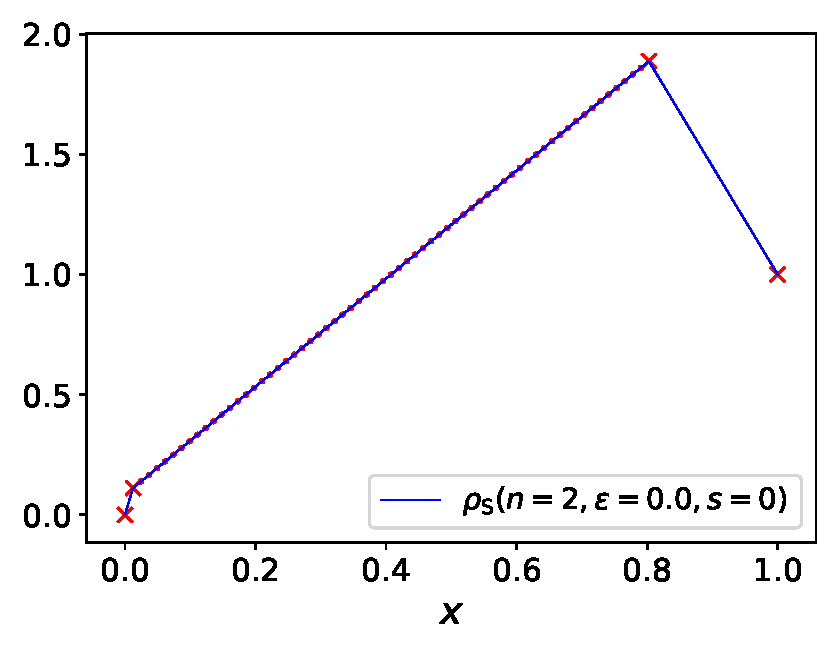
\includegraphics[scale=0.6]{figs/lcpoints.pdf}
    \caption{\textbf{All points on the Lorenz curve are uniformly distributed.}
    \cref{eq:x,eq:l}) capture the coordinates of all points up to the maximum.
    }
    \label{fig:lc}
\end{figure}

Consider the state 
\begin{equation*}
\rho_{\rm{S}}(n', \epsilon, n-n') \coloneqq \rho_{\rm{S}}(\epsilon)^{\otimes n'} \otimes \left( \frac{1}{3}\id \right)^{\otimes (n-n')},
\end{equation*}

Tensoring with the maximally mixed state keeps the Lorenz curve unchanged, but increases the resolution of (the uniformly distributed) points.
The new point coordinates are given by:
\begin{align}
    &x_{ijk} = \left( 1-p_{ijk}\right) x_{i-1} + p_{ijk} x_{i} \label{eq:lcsu_xcoord}\\
    &L_{ijk} = \left( 1-p_{ijk} \right) L_{i-1} + p_{ijk} L_{i}, \label{eq:lcsu_lcoord}\\
    &\text{where } p_{ijk} = \frac{k + (j-1)9^{n-n'}}{9^{n-n'} m_{i}} \nonumber\\
    &\text{for } i=0,\dots,n',\ j = 1,\dots,m_{i}(n', \epsilon') \text{ and } k = 1,\dots,9^{n-n'}. \nonumber
\end{align}

We can unify the indices, by introducing a single index
\begin{equation}
    I(i,j,k) \coloneqq k + \left[ (j-1) + \sum_{\ell=0}^{i-1} m_{\ell}(n', \epsilon') \right]9^{n-n'},
\end{equation}
so that $I=1,2,\dots, 9^{n}$.
The elbow coordinates correspond to 
\begin{equation}
	I(i, m_{i}(n', \epsilon'), 9^{n-n'}) = \sum_{\ell=0}^{i} m_{\ell}(n', \epsilon'),\ i= 0,\dots,n'.
\end{equation}
The index function $I$ is bijective, i.e.
\begin{equation}
	(i,j,k) = (i',j',k') \Leftrightarrow I(i,j,k) = I(i',j',k').
\end{equation}

\subsection{Strange state MSD in the unital fragment}\label{app:lc_compare}
Consider the Strange state MSD process in the unital fragment,
\begin{equation}\label{eq:su_conversion}
    \rho_{\rm{S}}(n', \epsilon, 0) \xrightarrow{\mathcal{O}_{\id/3}} \rho_{\rm{S}}(n', \epsilon', n-n').
\end{equation}
We denote initial state indices without a prime and target state indices with a prime,
\begin{align}
    I(i,j,k=1) &= j + \sum_{\ell=0}^{i-1} m_{\ell}(n, \epsilon), \\
    I'(i',j',k') &= k' + \left[ (j'-1) + \sum_{\ell=0}^{i'-1} m_{\ell}(n', \epsilon') \right]9^{n-n'}.
\end{align}

Pointwise Lorenz curve comparison requires $x_{I} = x_{I'}$, so the question is: 
\begin{center}
\emph{Given a triplet $(i',j',k')$, what is the tuple $(i,j)$ such that $I(i,j) = I'(i',j',k')$?}
\end{center}

According to~\cref{thm:elbows} which is proved in~\cref{app:lc_constraints}, for standard Lorenz curves, we need to match indices at the target state elbows, so the requirement on the indices is finding a tuple $(i, j)$, such that for a given $i' = 0,\dots,n'$,
\begin{equation}
	j + \sum_{\ell=0}^{i-1} m_{\ell}(n, \epsilon) = \sum_{\ell=0}^{i'} m_{\ell}(n', \epsilon').
\end{equation}

As a basic example, consider the process 
\begin{equation}
\rho_{\rm{S}}(\epsilon)^{\otimes 4} \xrightarrow{\mathcal{O}_{\id/3}} \rho_{\rm{S}}(\epsilon')^{\otimes 2} \otimes \left( \frac{1}{3}\id \right)^{\otimes 2}.
\end{equation}
We want to check which Lorenz curve is higher at the first elbows of the target state, i.e. we want to verify or reject the first inequality below:
\begin{equation}
	L_{I(i,j)} \geq L'_{I'(0, 1, 81)}
\end{equation}
where the first multiplicity of the target state is $m_0 = 1$.
The multiplicities of the initial state are $(1, 384, 4096)$.

The challenge is to find $i,j$ such that $i(i,j) = i'(0,1,81)$.
\nick{By trial and error}, we find that $(i,j) = (1, 80)$.
Now we can use~\cref{eq:lcsu_lcoord} to directly calculate
\begin{align*}
	L'_{i'(0,1,81)} &= L'_0 = \left( \frac{5}{3} - \frac{8}{9}\epsilon\ \right)^2 \Phi_+\left(0;2,4\frac{3-\epsilon}{15-8\epsilon}\right), \\
	L_{i(1, 80)} &= \left(1-\frac{80}{384} \right) L_0 + \frac{80}{384} L_1 \\
	\begin{split}
	&= \left( \frac{5}{3} - \frac{8}{9}\epsilon\ \right)^4 \bigg[ \frac{19}{24} \Phi_+\left(0;4,4\frac{3-\epsilon}{15-8\epsilon}\right) \\ 
	&\qquad + \frac{5}{24}\Phi_+\left(2;4,4\frac{3-\epsilon}{15-8\epsilon}\right) \bigg],
	\end{split}
\end{align*}
and then compare them.

%%%%%%%%%%%%%%%%%%%%%%%%%%%%%%%%%%%%%%%%

\section{Technical details of bound derivation in stabiliser fragments}
\label{app:lcst_technical}

\subsection{Component-multiplicity pairs}
\label{app:cmpairs}

In general, a $1$-copy $d$-dimensional state is defined exactly by its $d^2$ Wigner distribution $W$. 
The distribution $W$ can always be described by a Wigner-component vector $\bmw = (w_i)_{i=1,\dots,D}$ and a multiplicity vector $\bmm = (m_i)_{i=1,\dots,D}$, where $D \leq d^2$ and they form component-multiplicity pairs denoted by $\{(w_i, m_i)\}_{i=1,\dots,D}$.
\begin{definition}
	Consider a $d^2$-dimensional distribution $W$ and a positive integer $D$. 
	We call the set of order pairs $\{(w_i, m_i)\}_{i=1,\dots,D}$ a \emph{complete set of component-multiplicity pairs}, if $W$ contains $m_i$ components $w_i$ and $\sum_{i=0}^D m_i = d^2$.
\end{definition}
Therefore, such a set that describes a distribution $W$ contains in its description each component of $W$ exactly once.
As an example, two complete sets of pairs for the Strange state are $\{( -1/3, 1), ( 1/6, 8)\}$ and $\{(-1/3, 1), (1/6, 2), (1/6, 3), (1/6, 3)\}$.

Consider two states $\rho_A, \rho_B$ with Wigner distributions $\W{\rho_A}, \W{\rho_B}$ described respectively by complete sets of component-multiplicity pairs 
\begin{equation}
	\{(w_i, m_i)\}_{i=1,\dots,D_A} \text{ and } \{(w_j', m_j')\}_{j=0,\dots,D_B}.
\end{equation}
The multiplicative property of the Wigner distribution over a composite phase space $\cal{P}_{d_A} \times \cal{P}_{d_B}$ shown in~\cref{thm:wstate},
\begin{equation}
	\W[\bmx_A \oplus \bmx_B]{\rho_A \otimes \rho_B} = \W[\bmx_A]{\rho_A}\W[\bmx_B]{\rho_B},
\end{equation}
implies that the distribution $\W{\rho_A \otimes \rho_B}$ is $d_A^2 d_B^2$-dimensional and contains components of the form $w_i w_j'$. 
Therefore, the set $\{(w_i w_j', m_i m_j')\}$ with $i=1,\dots,D_A$ and $j=1,\dots,D_B$ is a complete set of component-multiplicity pairs for the distribution of the composite system $\W{\rho_A \otimes \rho_B}$.
This is true because all components are of the form $w_i w_j'$ and 
\begin{equation*}
	\sum_{i=1}^{D_A}\sum_{j=1}^{D_B} m_i m_j' = \sum_{i=1}^{D_A} m_i \sum_{j=1}^{D_B} m_j' = d_A^2 d_B^2.
\end{equation*}

Note that the rescaled distribution is also multiplicative,
\begin{align}
	&\widetilde{\rm{W}}_{\rho_A \otimes \rho_B | \gamma_A \otimes \gamma_B}(\bmx_A \oplus \bmx_B) = \frac{\W[\bmx_A \oplus \bmx_B]{\rho_A \otimes \rho_B}}{\W[\bmx_A \oplus \bmx_B]{\gamma_A \otimes \gamma_B}} = \nonumber \\
	&\frac{\W[\bmx_A]{\rho_A}\W[\bmx_B]{\rho_B}}{\W[\bmx_A]{\gamma_A}\W[\bmx_B]{\gamma_B}} = \widetilde{\rm{W}}_{\rho_A | \gamma_A}(\bmx_A)\widetilde{\rm{W}}_{\rho_B  | \gamma_B}(\bmx_B),
\end{align}
so result holds for this too \nick{FIX SECTION}.

Given a state $\rho$ and a complete set of component-multiplicity pairs describing its Wigner distribution $\W{\rho}$, we now provide a method of computing the components (and multiplicities) of the $n$-copy distribution $\W{\rho}^{\otimes n}$.
\begin{lemma}\label{lem:ncopycomponents}
	Let $W$ be a $d$-dimensional distribution defined by a complete set of component-multiplicity pairs $\{(w_i, m_i)\}_{i=1,\dots,D}$ with $D \leq d$ and consider the distribution $W^{\otimes n}$ obtained by taking the Kronecker product $W \otimes \dots \otimes W$ between $n$ copies of $W$.
	
	Denote by $C_D^n \coloneqq \{\bmk\}$ the set of all vectors $\bmk \coloneqq (k_1, \dots, k_D)$ with non-negative integer components that sum to $n$, i.e.
	\begin{equation*}
	0 \leq k_1, \dots, k_D \leq n \text{ and } k_1 + \dots + k_D = n.
	\end{equation*}
	
	Then, $W^{\otimes n}$ admits a complete set of component-multiplicity pairs $\{(W_{\bmk}, M_{\bmk})\}_{\bmk \in C_D^n}$, where
\begin{align}
	M_{\bmk} &= \frac{n!}{k_1!\dots k_D!} \prod\limits_{i=1}^D {m_i}^{k_i}, \label{eq:M}\\
	W_{\bmk} &= \prod\limits_{i=1}^D {w_i}^{k_i}. \label{eq:W}
\end{align}
\end{lemma}
\begin{proof}
	We proceed by induction.
	
	Assume $n = 1$.
	Let $\bmk_i \coloneqq (0,\dots,0,1,0,\dots,0)$ be a vector with its $i$-th component equal to 1 and 0's elsewhere.
	The set $C_D^1$ consists of all vectors of this form, i.e. 
\begin{equation*}
	C_D^1 = \{ \bmk_i \}_{i=1,\dots,D}
\end{equation*}
	It is also true by direct calculation that
\begin{equation*}
	\left( W_{\bmk_i}, M_{\bmk_i} \right) = (w_i, m_i).
\end{equation*}
Therefore, $\{ (W_{\bmk}, M_{\bmk}) \}_{\bmk \in C_D^1}$ is a complete set of component-multiplicity pairs for $W$.

	Assume that $\{(W_{\bmk}, M_{\bmk})\}_{\bmk \in C_D^n}$ as given in~\cref{eq:M,eq:W} is a complete set of component-multiplicity pairs for the $n$-copy distribution $W^{\otimes n}$.
	By construction, the distribution $W^{\otimes (n+1)} = W^{\otimes n} \otimes W$ is multiplicative, so it admits the complete set of component multiplicity pairs
\begin{equation}
	\{(W_{\bmk} w_i, M_{\bmk} m_i)\},\ \bmk \in C_D^n \text{ and } i=1,\dots,D.
\end{equation}
	
	Consider the component sum of the distribution $W^{\otimes (n+1)}$,
\begin{align*}
	&\sum_{\bmk \in C_D^n}\sum_{i=1}^D M_{\bmk} m_i W_{\bmk} w_i = \sum_{\bmk \in C_D^n} M_{\bmk}W_{\bmk} \sum_{i=1}^D m_i w_i =\\
	&\sum_{\bmk \in C_D^n} \frac{n!}{k_1!\dots k_D!} \prod\limits_{i=1}^D {m_i}^{k_i}{w_i}^{k_i} \sum_{i=1}^D m_i w_i =\\
	&\left( \sum_{i=1}^D m_i w_i \right)^n \left( \sum_{i=1}^D m_i w_i \right) = \left( \sum_{i=1}^D m_i w_i \right)^{n+1} =\\
	&\sum_{\bmq \in C_D^{n+1}} M_{\bmq}W_{\bmq},
\end{align*}
where in the last expression, vectors $\bmq = (q_1, \dots, q_D)$ have non-negative integer components that sum to $(n+1)$ and 
\begin{align*}
	M_{\bmq} &= \frac{(n+1)!}{q_1!\dots q_D!} \prod\limits_{i=1}^D {m_i}^{q_i},\\
	W_{\bmq} &= \prod\limits_{i=1}^D {w_i}^{q_i}.
\end{align*}
We have used the multinomial theorem to proceed between lines 2-3 and lines 3-4 of the derivation.

We have achieved a regrouping of the distribution components.
Every component $W_{\bmq}$ is of the form $W_{\bmk} w_i$ with $q_i = k_i + 1$ and $q_j = k_j$ for $j\neq i$ and 
\begin{align*}
	\sum_{\bmq \in C_D^{n+1}}  \hspace{-6pt} M_{\bmq} =  \hspace{-10pt} \sum_{\bmq \in C_D^{n+1}} \frac{(n+1)!}{q_1!\dots q_D!} \prod\limits_{i=1}^D {m_i}^{q_i} = 
	\left( \sum_{i=1}^D m_i \right)^{n+1} \hspace{-10pt} = d^{n+1},
\end{align*}
which is the dimension of $W^{\otimes (n+1)}$.

Therefore, $\{ (W_{\bmq}, M_{\bmq}) \}_{\bmq \in C_D^{n+1}}$ is a complete set of component-multiplicity pairs for $W^{\otimes n}$, completing the proof.
\end{proof}

\subsection{First elbow location}
\label{app:first_elb_loc}

Here, we show that the horizontal location of the first elbow is lower for an initial state compared to the target state for a valid distillation process ($n > n'$).
\begin{enumerate}
	\item $\rm{(C1)} \rightarrow \rm{(C1)}$. 
	It is always true that $e^{-\beta E_0} / \Z_\beta \leq 1$, so
	\begin{align*}
		x_0 &= \left(\dfrac{e^{-\beta E_0}}{3\Z_\beta}\right)^n = \left(\dfrac{e^{-\beta E_0}}{3\Z_\beta}\right)^{n-n'} \left(\dfrac{e^{-\beta E_0}}{3\Z_\beta}\right)^{n'} \\
		&< \left(\dfrac{e^{-\beta E_0}}{3\Z_\beta}\right)^{n'} = x_0'		
	\end{align*}
	\item $\rm{(C2)} \rightarrow \rm{(C1)}$.
	It is always true that
	\begin{align*}
		&\Z_\beta^{n-n'} > (e^{-\beta E_{\rm{max}}})^{n-n'} = e^{-\beta (n-n') E_{\rm{max}}}, \text{ so} \\
		x_0 &= \left(\dfrac{e^{-\beta E_{\rm{max}}}}{\Z_\beta}\right)^n = \dfrac{e^{-\beta(n E_{\rm{max}} - n' E_0)}}{\Z_\beta^{n-n'}} \left(\dfrac{e^{-\beta E_0}}{3\Z_\beta}\right)^{n'} \\
		&< \dfrac{e^{-\beta(n E_{\rm{max}} - n' E_0)}}{e^{-\beta (n-n') E_{\rm{max}}}} \left(\dfrac{e^{-\beta E_0}}{3\Z_\beta}\right)^{n'} \\
		&= e^{-\beta n' (E_{\rm{max}} - E_0)} \left(\dfrac{e^{-\beta E_0}}{3\Z_\beta}\right)^{n'} \\
		&\leq \left(\dfrac{e^{-\beta E_0}}{3\Z_\beta}\right)^{n'} = x_0'.
	\end{align*}
	\item $\rm{(C2)} \rightarrow \rm{(C2)}$.
	It is always true that $e^{-\beta E_{\rm{max}}} / \Z_\beta \leq 1$, so
	\begin{align*}
		x_0 &= \left(\dfrac{e^{-\beta E_{\rm{max}}}}{\Z_\beta}\right)^n = \left(\dfrac{e^{-\beta E_{\rm{max}}}}{\Z_\beta}\right)^{n-n'} \left(\dfrac{e^{-\beta E_{\rm{max}}}}{\Z_\beta}\right)^{n'} \\
		&\leq \left(\dfrac{e^{-\beta E_{\rm{max}}}}{\Z_\beta}\right)^{n'} = x_0'	
	\end{align*}
\end{enumerate}



























